\documentclass{article}
\usepackage{geometry}
\usepackage[T1]{fontenc}
\usepackage[utf8]{inputenc}
\usepackage{amssymb}
\usepackage{amsmath}
\usepackage{german}
\usepackage{tikz}
\usepackage{fancybox}

\geometry{a4paper, left=40mm, right=30mm, top=30mm, bottom=30mm}

\begin{document}
	 
	 \section{Baum}
	 \begin{enumerate}
	 	\item Baum besteht aus Knoten (Kreise) und Kanten (Pfeile)
	 	\item Kanten verbinden Knoten mit ihren Kind-Knoten
	 	\item jeder Knoten (außer der Wurzel) hat \underline{genau ein} Elternteil
	 	\item Knoten ohne Kinder heißen "Blätter" $(leaf - nodes)$
	 	\item Teilbaum
	 	\begin{enumerate}
	 		\item wähle beliebigen Knoten
	 	\end{enumerate}
	 \end{enumerate}
	 
	 Infix Notation: \\
	 $1+2+3*4/(1+5)-2$ \\ \\
	 
	 Präfix Notation: \\
	 $sub(add(add(1,2), div(mul(3,4), add(1,5))),2)$ \\ \\
	 
	 
	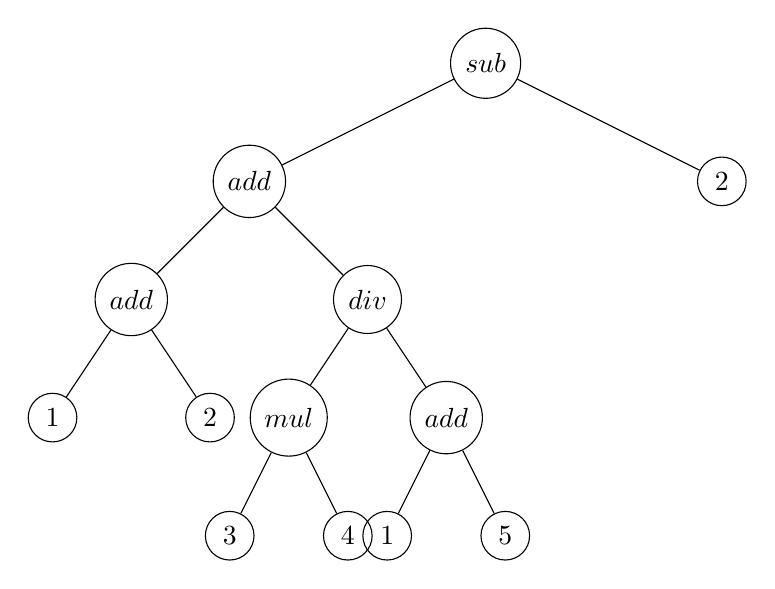
\begin{tikzpicture}[level/.style={sibling distance=60mm/#1}]
	
	\node [circle, draw] (z)  {$sub$}
	child {node [circle, draw] {$add$}
		child {node [circle, draw] {$add$}
			child{node [circle, draw] {$1$}}
			child{node [circle, draw] {$2$}}
		}
		child {node [circle, draw] {$div$}
			child{node [circle, draw] {$mul$}
				child {node [circle, draw] {$3$}}
				child {node [circle, draw] {$4$}}
			}
			child{node [circle, draw] {$add$}
				child {node [circle, draw] {$1$}}
				child {node [circle, draw] {$5$}}
			}
		}}
	child {node [circle, draw] {$2$}
	};
	\end{tikzpicture}
	
	\paragraph{Präfix Notation aus dem Baum rekonstruieren}
	
	\begin{enumerate}
		\item Wenn die Wurzel ein Blatt ist, dann "Drucke die Zahl"
		\item sonst $(Operator):$
		\begin{enumerate}
			\item Drucke Funktionsnamen
			\item Drucke \"(\"
			\item wiederhole ab 1) für das linke Kind
			\item Drucke $,$
			\item wiederhole den Algorithmus ab $1)$ für das rechte Kind
			\item Drucke \")\"
		\end{enumerate}
 	\end{enumerate}
 	
 	Beachte Reihenfolge: Wurzel - Links - Rechts (Pre-Order Traversal)
		Ergebnis: \\
		$sub(add(add(1,2), div(mul(3,4), add(1,5))),2)$

	\paragraph{Definition: Rekursion}
		Rekursion meint Algorithmus für Teilproblem von vorn
		
	\paragraph{Infix Notation}
	
	\begin{enumerate}
		\item wie bei Präfix
		\item sonst
		\begin{enumerate}
			\item entfällt
			\item wie bei Präfix
			\item wie bei Präfix
			\item Drucke Operatorsymbol
			\item wie bei Präfix 
			\item wie bei Präfix
			\item wie bei Präfix
		\end{enumerate}
	\end{enumerate}
	 	Beachte Reihenfolge: Links - Wurzel - Rechts (In-Order Traversal) \newline
	 	
		Ergebnis: \\
		$(((1 + 2) + ((3 * 4)/(1 + 5))) + 2)$
	
	\paragraph{Berechne den Wert mit Substitutionsmethode}
		\begin{enumerate}
			\item Wenn Wurzel ein Blatt hat, gib die Zahl zurück
			\item sonst
			\begin{enumerate}
				\item entfällt
				\item entfällt
				\item wiederhole ab $1)$ für linken Teilbaum und speichere Ergebnis als $"left-result"$
				\item entfällt
				\item wiederhole ab $1)$ für rechten Teilbaum, speichere Ergebnis als $"right-result"$
				\item berechne $fkt_name(left-result, right-result)$ und gib Ergebnis zurück
			\end{enumerate}
		\end{enumerate}
		Beachte Reihenfolge: Links - Rechts - Wurzel (Post-Order Traversal)
		
		\begin{align*}
			&  	sub(add(add(1,2), div(mul(3,4), add(1,5))),2) \\
			= & \, sub(add(add(1,2), div(12, 6)),2) \\
			= & \, sub(add(3,2)2) \\
			= & \, sub(5,2) \\
			= & \, 3
		\end{align*}
		
		\chapter{Maschinensprache}
		\begin{itemize}
			\item optimiert für die Hardware (viele verschiedene)
			\item Gegensatz: höhere Programmiersprache ($C++$) ist optimiert für Programmierer
			\item Compiler oder Interpreter übersetzen Hoch- in Maschinensprache 
		\end{itemize}
		
		\paragraph{Vorgang des Übersetzens}
		\begin{enumerate}
			\item Eingaben (und Zwischenergebnisse) werden in Speicherzellen abgelegt $ \Rightarrow$ jeder Knoten im Baum bekommt eine Speicherzelle (Maschinensprache: durchnumeriert ; Hochsprache: sprechende Namen)
			\item Speicherzellen für die Eingaben $\underline{initialisieren}$ ; Notation: SpZ $\leftarrow$ Wert
			\item Rechenoperationen in der Reihenfolge des Substitutionsmodells ausführen und in der jeweiligen Speicherzelle speichern ; Notation: SpZ\_Ergebnis $\leftarrow$ fkt\_name SpZ\_Arg1 SpZ\_Arg2
			\item alles in Zahlencode umwandeln
			\begin{itemize}
				\item Funktionsname $\Rightarrow$ Opcodes
				\item Speicherzellen: nur die Nummer
				\item Werte sind schon Zahlen
				\item Notation: Opcode \quad Ziel SpZ \quad SpZ\_Arg1 \quad SpZ\_Arg2 oder Opcode \quad Ziel SpZ \quad Initialwert
				
			\end{itemize}
		\end{enumerate}
		
	
\end{document}